\chapter{Runtime Energy Profiling and Threshold Adaptation}

% Nickname
\newcommand{\nn}{\textsc{Opta}}

\section{Introduction}

% *** Background of energy harvesting and intermittent systems ***

Energy harvesting has become a promising power solution for the Internet of Things, liberating wireless sensors from batteries and the power grid. 
Batteryless devices harvest ambient energy, such as light, radio-frequency, and mechanical movement, which is then buffered in a capacitor. 
As the harvested power is typically insufficient for continuous operation, such devices operate in an intermittent way -- when a certain amount of energy is collected, the processor wakes up, executes program until the amount of energy falls below a threshold, where it sleeps or dies, and waits for the next energy cycle [ref]. 
Prior work in \textit{intermittent systems} has developed sophisticated methods to preserve forward progress across frequent power interruptions by carefully \textit{checkpointing} the volatile computing state in CPU registers and volatile memory into non-volatile memory (NVM), and restoring it on reboot [ref]. 


% *** Previous work on intermittent peripheral operations ***

Apart from computing, embedded sensor systems need to utilize peripherals, such as sensors, computational accelerators, and radios, which typically require \textit{atomicity}.
In the context of intermittent systems, an atomic operation should not be checkpointed during execution; if interrupted by power failures, it should restart rather than checkpoint and resume.
A peripheral operation is considered atomic because it is infeasible to completely read, save, and restore the intermediate internal state of peripherals, and even if possible, could produce unwanted results. 
% Need elaboration
(Example)
% disable checkpoints during execution
Prior works on intermittent peripheral operations either individually dedicate an  design-time calibrated energy budget for each peripheral operation~\cite{gomez2016dynamic}, or allocate a universal energy budget that ensure the most energy hungry operation can finish in one energy cycle~\cite{maeng2019supporting}.



% *** Offline profiling and fixed threshold is impractical due to variability ***

However, in this paper we propose that manually profiling each peripheral operation and setting fixed thresholds is impractical due to variability in capacitance and energy consumption, where we have considered the following cases: 

\begin{enumerate}
    \item \textit{Variability in capacitance:} 
    As a component for buffering energy in intermittent systems, capacitors typically present a $\pm$10-20\% tolerance on rated capacitance. 
    Capacitors also age over time. 
    It is shown that capacitance can decrease by 7.2\% in 3000 hours under a \SI{25}{\celsius} ambient temperature in experiments~\cite{kulkarni2010experimental}, and by 50\% within 10 years under \SI{40}{\celsius} as manufacturers stated~\cite{vishaycapacitor}.
    A degraded capacitor does not change the load consumption, but can increase the voltage difference before and after an operation, and hence makes the pre-defined voltage threshold unsafe. 

    \item \textit{Variable amount of data to process:}
    A peripheral function can accept a runtime variable amount of data, e.g. sending different lengths of packets or encrypting different amount of data. 
    Statistically, this linearly scales the charge consumption.

    \item \textit{Variability in peripheral configurations:}
    A peripheral can run with variable configurations at runtime, and demonstrate variable performance and energy consumption. 
    For example, an AES accelerator can encrypt or decrypt data with 128-, 192-, or 256-bit keys. 
    A longer key provides more security, but also takes more time and energy to complete.
    % Can refer to "A control flow" for the need of runtime configurations

    \item \textit{Device variability:}
    Devices have their variation in power consumption, even with the same part number. 
    A threshold profiled on one device can be inadequate on another. 
\end{enumerate}

A fixed threshold can be violated if any of the above cases happen, and lead to non-termination. 
In practical deployment, profiling every atomic operation for every device with all runtime scenarios could an extremely tedious work.
Considering this complexity, it is unrealistic to profile the energy budget in every scenario and customize a voltage threshold accordingly. 



% *** An optimized threshold improves efficiency ***

On the other hand, using only one high voltage threshold, though probably avoids non-termination, can affect system efficiency. Microcontrollers and peripheral devices typically draw more current at a higher supply voltage. The high voltage in the buffering capacitor can also decrease the charging efficiency of energy harvesters and increase system leakage. Hence, setting a high voltage threshold for the processor to wake up results in a superlinear long charging time, which therefore slows down the system execution or even leave the system in a infinite wait at low input power. 


% *** What we do to address it ***

To address the above issue, we propose \nn{} (online profiling and threshold adaptation), a methodology that profiles energy consumption of operations at runtime and allocate adaptive thresholds based on newly profiled consumption and user-defined parameters. 
\nn{} profiles the voltage decrease that an operation can cause without any energy input during the operation, while the energy harvesting supply is connected. 
The profiling strategy is to measure the input current in the charging cycle so as to calculate the maximum drop of supply voltage in the discharging cycle. 
The profiled energy budget can therefore guarantee the completion of an atomic operation. 
Based on the profiling results, \nn{} dynamically adapts the threshold for each atomic operation, with an option of scaling threshold by user-defined parameters or peripheral configurations.



*** Contributions and paper structure ***



\section{Background and Motivation}


% Outline
% Review the profiling methods/concepts in prior work.
% Peripheral papers
%   1. How they manage to do peripheral operations?
%   2. Are they supposed to fail in our scenarios?


\subsection{Intermittent Peripheral Operations}

% Intro
% While prior work in intermittent computing have been able to efficiently maintain forward progress on computational workloads, intermittent peripheral operations are not widely studied. 
% This is typically achieved by carefully saving volatile computing state (e.g. data in CPU registers, SRAM) into NVM before a power failure, and restoring it on power recovery. 
% Some of the published approaches intrinsically guarantee the atomicity and termination of peripheral operations, while others focus on computational workloads without support for peripherals. 
Several papers have been published on handling atomic peripheral operations in intermittent systems, where energy profiling of workloads is an inherent part of their methodologies.

% Review of papers about or support peripherals
%   Karma? Sytare?

% DEBS
DEBS~\cite{gomez2016dynamic} experimentally profiles the energy consumption of each task at design time, and designates a threshold to each task individually.
DEBS enters a low-power mode (LPM) after completing an operation, and waits for energy replenishment until the next threshold. 

% Samoyed, Alpaca?
Samoyed~\cite{maeng2019supporting} utilizes a custom design-time \textit{energy profiler}~\cite{colin2016energy-interference-free} to identify whether the adopted energy storage size suffices to run an adequate number (hundreds, as suggested) of peripheral operations in one energy cycle. 
At runtime, Samoyed starts execution when energy is refilled to a certain threshold, and keeps executing until energy is depleted. 
% Samoyed is a proactive approach where the program knows the boundaries of atomic operations, such that it only outputs valid data on the completion of an atomic operation and disables checkpoints during execution. 
Samoyed differs from most static approaches, e.g. Alpaca, on handling computational workloads where it reactively checkpoints when energy falls below a low threshold, and supports user-customized subdivision of peripheral operations when the operation cannot complete in one energy cycle. 

% RESTOP (similar to re-execution)
RESTOP~\cite{rodriguez2018restop} provides programmer-configurable rules that track the instructions issued to peripherals through serial interfaces in a history table.
On power recovery, RESTOP re-issues instructions saved in the history table and then resumes the interrupted operation. 
At design time, RESTOP needs to profile the worst-case energy consumption for restoring peripheral state to identify the minimum (most-efficient) restore threshold. 

% Adaptive?
% Online profiling but inefficient



Prior work profiles the energy consumption of each atomic operation at design time to determine a voltage threshold or a capacitor size that ensures forward progress. 
However, this does not guarantee the completion of every atomic operation because energy consumption can change with any runtime conditions different to the profiling setup (detailed in Section~\ref{subsec:dynamic_energy_consumption}). 
Hence, previous designs typically achieve atomicity by carefully managing the system state, such that the atomic operation does not output valid data until completion, and, if a power failure happens during the operation, the system state rolls back to the start of the operation upon power recovery (rather than checkpoint and resume). 
Also, previous designs should usually leave an inefficiently safe margin between the profiled energy consumption and the energy to be allocated, such that dynamic variation can be largely tolerated. 



% Comments: 
% All previous work involves a design-time energy profiling of workloads.




% Comments: Justify Samoyed, DEBS for comparisons in this paper? 

\subsection{Variability in Energy Consumption, Storage, and Input} \label{subsec:dynamic_energy_consumption}


We took an example of atomic operations to study the dynamic variation of energy consumption. We chose the AES accelerator on TI MSP430FR5994, running a data encryption peripheral function. 

Explain each kind of dynamic variation of energy consumption, as listed in Section I-A.

\subsubsection{Capacitor Degradation and Tolerance}

\subsubsection{Data size}


\begin{figure}[!t]
    \centering
    \begin{tikzpicture}
    \begin{axis}[
            width=1.0\columnwidth,
            height=5cm,
            ymin=0,
            ymax=200,
            xmin=0,
            xmax=4,
            xlabel=Data Size (KiB),
            ylabel=$\Delta V_{\text{task}}$ (mV),
            legend style={at={(0.05,0.95)},
            anchor=north west,legend columns=1},
        ]
        \addplot
            plot [black,only marks]
            table [x=data_size, y=voltage_drop,col sep=comma] {ch5_repta/figures/variable_data/variable_data.csv};
        \addplot
            plot [black]
            {44.3 * x + 16.9};
        \legend{Measurements, Linear Fit}
    \end{axis}
    \end{tikzpicture}
    \caption{Voltage drop vs data size.}
    \label{fig:variable_datasize}
\end{figure}

Figure~\ref{fig:variable_datasize}

\subsubsection{Peripheral Configurations}

Table~\ref{tab:configurations}

\begin{table}[!t]
    \renewcommand{\arraystretch}{1.2}
    \centering
    \caption{Peripheral configuration variability, AES Encryption 4KB}
    \label{tab:configurations}
    \begin{tabular}{|c|c|}
    \hline
    \textbf{Configuration} & \textbf{$\Delta V_{\text{task}}$}\\
    \hline
    128-bit key & \SI{194}{\milli\volt}\\
    192-bit key & \SI{230}{\milli\volt}\\
    256-bit key & \SI{245}{\milli\volt}\\
    \hline
    \end{tabular}
\end{table}

\subsubsection{Device}

Table~\ref{tab:device}

\begin{table}[!t]
    \renewcommand{\arraystretch}{1.2}
    \centering
    \caption{Device variability, AES 128-bit Encryption 4KB}
    \label{tab:device}
    \begin{tabular}{|c|c|c|c|}
    \hline
    \textbf{Device No.} & \textbf{$\Delta V_{\text{task}}$} & \textbf{System Capacitance} & \textbf{Time} \\
    \hline
    % 1 & \SI{764}{\micro\ampere}\\
    % 2 & \SI{773}{\micro\ampere}\\
    % 3 & \SI{756}{\micro\ampere}\\
    1 & \SI{185}{\milli\volt} & \SI{29}{\micro\farad} & \SI{6.444}{\milli\second} \\
    2 & \SI{194}{\milli\volt} & \SI{35}{\micro\farad} & \SI{6.479}{\milli\second} \\
    3 & \SI{179}{\milli\volt} & \SI{29}{\micro\farad} & \SI{6.462}{\milli\second} \\
    \hline
    \end{tabular}
\end{table}

\subsubsection{Other}
Clock frequency (Tentative). 1MHz: 757uA (This should be checked later as it takes the same time to complete).

% \subsection{To operate at a lower voltage}

\subsubsection{Voltage}

(This should be relevant as you mention it's better to operate at lower voltage)


% Prior experiment

% 2.1V: 750uA

% 2.4V: 755uA

% 2.7V: 763uA

% 3.0V: 763uA

% 3.3V: 764uA

% 3.6V: 764uA


% New experiment

| Start V | End V | Delta V |

| 2.020V        | 1.836V      | 184mV   |

| 2.102V        | 1.917V      | 185mV   |

| 2.214V        | 2.030V      | 184mV   |

| 2.301V        | 2.117V      | 184mV   |

| 2.424V        | 2.240V      | 184mV   |

| 2.542V        | 2.352V      | 190mV   |

| 2.634V        | 2.444V      | 190mV   |

| 2.710V        | 2.521V      | 189mV   |

| 3.360V        | 3.166V      | 194mV   |

% Figure~\ref{fig:voltage}
% \begin{figure}[!h]
%     \centering
%     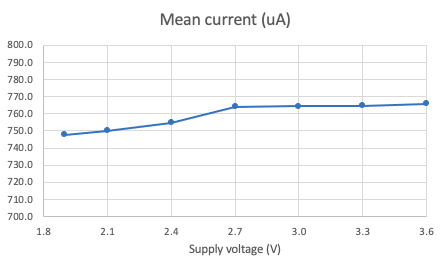
\includegraphics[width=3.49in]{voltage.jpg}
%     \caption{Current consumption vs voltage. }
%     \label{fig:voltage}
% \end{figure}

\subsubsection{Charging efficiency of energy harveser vs Vcc}

\begin{figure}[!t]
    \centering
    \begin{tikzpicture}
    \begin{axis}[
            width=1.0\columnwidth,
            height=5cm,
            ymin=0,
            ymax=130,
            xmin=0,
            xmax=5.3,
            xlabel=Voltage (V),
            ylabel=Current (\SI{}{\micro\ampere}),
            legend style={at={(0.05,0.05)},
            anchor=south west,legend columns=1},
        ]
        \addplot
            plot [black,only marks]
            table [x=v, y=i,col sep=comma] {ch5_repta/figures/pv_curve/pv_curve.csv};
        \addplot
            plot [black,ultra thick]
            {-7.2 * x + 124.4};
        \legend{Measurements, Linear Fit for \SIrange{0}{4}{\volt}}
        % \legend{Measurements}
    \end{axis}
    \end{tikzpicture}
    \caption{IV curve.}
    \label{fig:pv_iv}
\end{figure}


% \subsection{Infeasibility Offline Profiling}

% As shown in Section~\ref{subsec:dynamic_energy_consumption}, dynamic current consumption is in existence across the variation of devices, clock frequencies, supply voltage, and temperature.





% Simulation
\subsection{Forward Progress Improvement with Adaptive Energy Budgeting}

We took a modelling process to demonstrate the potential of improving forward progress with adaptive energy budgeting, given dynamic execution time and dynamic current draw.

\subsubsection{Model Description}
We modelled an ideal case of adaptive energy budgeting, where the system exactly knows how much time the next atomic operation will take and how much the current draw is. The system sets a voltage threshold that exactly guarantees the charge consumption even if the supply current immediately drops to zero after the start of an operation. 

\subsubsection{Simulation Setup}
The system has a \SI{10}{\micro\farad} capacitor for buffering energy with \SI{1.5}{\volt} charge at the beginning. 
The system consumes \SI{20}{\micro\ampere} in the LPM and \SI{0}{\micro\ampere} when off.
The shutdown threshold is \SI{1.8}{\volt}, which is also the end voltage that all approaches are profiled for or adapted to. 
We set a dummy workload which draws \SI{750}{\micro\ampere} and takes up to \SI{5}{\milli\second} to complete.
Two sets of simulation were conducted.
One set was run with a randomized dynamic execution time that is uniformly distributed between 0 and \SI{5}{\milli\second}, with \SI{750}{\micro\ampere} current draw unchanged. The other was run with a dynamic current draw which is increased by 0-20\% uniformly distributed, with \SI{5}{\milli\second} execution time. 
We ran each set of simulation for 10 times and took the mean, maximum, and minimum of the number of completed operations as a metric of forward progress. 

\subsubsection{Results}

Figure~\ref{fig:model_time}.

\begin{figure}[t]
    \centering
    \begin{tikzpicture}
    \begin{axis}[
        width=1.0\columnwidth, height=5cm,
        ybar,
        ymin=0,
        ymax=600,
        enlarge x limits=0.3,
        legend style={at={(0.5,1.2)},
        anchor=north,legend columns=-1},
        ylabel={No. completions},
        symbolic x coords={\SI{100}{\micro\ampere},\SI{300}{\micro\ampere},\SI{500}{\micro\ampere}},
        xtick=data,
    ]
    % Samoyed
    \addplot
        plot [black,fill=Set1-A,postaction={pattern=dots},error bars/.cd,y dir=both,y explicit]
        table [x=current,y=samoyed_perf,y error plus=samoyed_perf_err+, y error minus=samoyed_perf_err-, col sep=comma] {ch5_repta/figures/model_time/model_time.csv};
    % DEBS
    \addplot
        plot [black,fill=Set1-B,postaction={pattern=north east lines},error bars/.cd,y dir=both,y explicit]
        table [x=current,y=debs_perf,y error plus=debs_perf_err+, y error minus=debs_perf_err-, col sep=comma] {ch5_repta/figures/model_time/model_time.csv};
    % Adaptive
    \addplot
        plot [black,fill=Set1-C,postaction={pattern=north west lines},error bars/.cd,y dir=both,y explicit]
        table [x=current,y=opta_perf,y error plus=opta_perf_err+, y error minus=opta_perf_err-, col sep=comma] {ch5_repta/figures/model_time/model_time.csv};
    \legend{Samoyed, DEBS, Adaptive}
    \end{axis}
    \end{tikzpicture}
    \caption{Dynamic execution time.}
    \label{fig:model_time}
\end{figure} 


Figure~\ref{fig:model_current}.
\begin{figure}[t]
    \centering
    \begin{tikzpicture}
    \begin{axis}[
        width=1.0\columnwidth, height=5cm,
        ybar,
        ymin=0,
        ymax=250,
        enlarge x limits=0.3,
        legend style={at={(0.5,1.2)},
            anchor=north,legend columns=-1},
        ylabel={No. completions},
        symbolic x coords={\SI{100}{\micro\ampere},\SI{300}{\micro\ampere},\SI{500}{\micro\ampere}},
        xtick=data,
        ]
        % Samoyed
        \addplot
            plot [black,fill=Set1-A,postaction={pattern=dots},error bars/.cd,y dir=both,y explicit]
            table [x=current,y=samoyed_perf,y error plus=samoyed_perf_err+, y error minus=samoyed_perf_err-, col sep=comma] {ch5_repta/figures/model_current/model_current.csv};
        % DEBS
        \addplot
            plot [black,fill=Set1-B,postaction={pattern=north east lines},error bars/.cd,y dir=both,y explicit]
            table [x=current,y=debs_perf,y error plus=debs_perf_err+, y error minus=debs_perf_err-, col sep=comma] {ch5_repta/figures/model_current/model_current.csv};
        % Adaptive
        \addplot
            plot [black,fill=Set1-C,postaction={pattern=north west lines},error bars/.cd,y dir=both,y explicit]
            table [x=current,y=opta_perf,y error plus=opta_perf_err+, y error minus=opta_perf_err-, col sep=comma] {ch5_repta/figures/model_current/model_current.csv};
        \legend{Samoyed, DEBS, Adaptive}
    \end{axis}
    \end{tikzpicture}
    \caption{Dynamic current draw.}
    \label{fig:model_current}
\end{figure} 
    

Analyse where the improvement comes from (probably with a voltage trace).
\newpage
\section{Methodology}

Motivated by the previous examples, we propose OPTA, a new methodology for profiling energy consumption of tasks at runtime and dynamically adapting the energy budget to the varying energy consumption of tasks. 

\subsection{Online Profiling Method}

Here, we present an efficient online profiling method. 
OPTA dynamically profiles the actual voltage droop that a task consumes while the supply is connected. 
The actual voltage droop means the voltage droop in ${V_{cc}}$ by running a task if the supply current immediately drops to zero after the task starts. 
With the supply connected, the supply current keeps charging the capacitor during execution, so the actual voltage droop cannot be measured simply by two voltage measurements at the beginning and the end of a task. 
A naive solution will be disconnecting or short-circuiting the supply during profiling, but this can waste energy. 
In contrast, while keeping the supply connected, our method analyzes the supply current in the charge cycle, and uses it to derive the actual voltage droop in the discharge cycle. 
We will explain this method with its mathematical reasoning first, and then discuss possible concerns in its implementation. 

\subsubsection{Assumptions}

We have made the following assumptions for the mathematical reasoning. Later, we will discuss the situations where these assumptions do not hold.

\begin{itemize}
    \item \textit{The supply current remains constant across a charge-discharge cycle.} 
    In intermittently-powered systems, the energy buffering capacitor is typically small, e.g. tens to hundreds of \SI{}{\micro\farad}, and hence the charge-discharge cycle is typically short, e.g. tens to hundreds of \SI{}{\milli\second}. 
    The supply current is unlikely to change in such a short period. 
    Hence, in the following reasoning, we presume that the supply current is constant across a charge-discharge cycle. 

    \item \textit{The system is able to measure the supply voltage and time when active.} Off-the-shelf MCUs, e.g. MSP430 series, are equipped with many low-power peripherals, including ADC for measuring voltage and RTC for time-keeping. 
    In the following reasoning, we assume that these two modules are available and free of any overheads.
\end{itemize}

\subsubsection{Mathmatical Derivation}

\begin{figure}[!t]
    \centering
    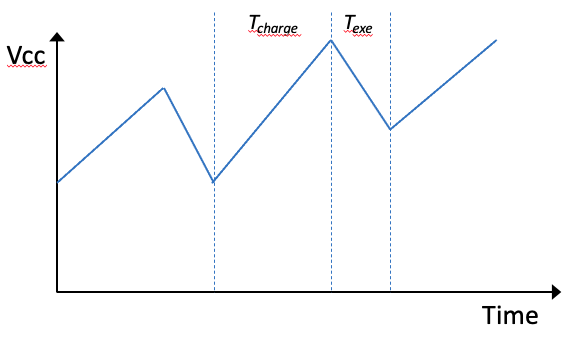
\includegraphics[width=3.49in]{ch5_repta/figures/math.jpg}
    \caption{Figure for illustrating mathematical derivation. }
    \label{fig:math}
\end{figure}

We show an illustrative trace of $V_{cc}$ across charge-discharge cycles in Fig.~\ref{fig:math}. 

(A list that explains math symbols to be inserted)

The charging cycle can be described as
\begin{equation}
    \Delta V_{charge} C = (I_{in} - I_{sleep}) T_{charge}
    \label{eq:vcharge} 
\end{equation}
where 
\begin{equation}
    I_{sleep} = I_{comp} + I_{rtc} + I_{lpm}
    \label{eq:isleep} 
\end{equation}

The discharging cycle can be described as
\begin{equation}
    \Delta V_{discharge} C = (I_{in} - I_{exe}) T_{discharge}
    \label{eq:vdischarge} 
\end{equation}
where
\begin{equation}
    I_{exe} = I_{comp} + I_{rtc} + I_{task}
    \label{eq:iexe} 
\end{equation}

The actual charge consumption of a task is
\begin{equation}
    \Delta V_{task} C = I_{exe} T_{discharge}
    \label{eq:vtaskc} 
\end{equation}

Combining (\ref{eq:vcharge}), (\ref{eq:isleep}), (\ref{eq:vdischarge}), (\ref{eq:iexe}), and (\ref{eq:vtaskc}), we can get the expression of $\Delta V_{task}$ as
\begin{equation}
    \Delta V_{task} = \Delta V_{charge} \frac{T_{exe}}{T_{charge}} - \Delta V_{exe} + \frac{I_{sleep}T_{exe}}{C}
    \label{eq:vtask} 
\end{equation}

Here, $\Delta V_{task}$ is the actual voltage droop that we should allocate before the execution of a task. 
$\Delta V_{charge}$, $\Delta V_{exe}$, $T_{exe}$, and $T_{charge}$ are the values that can be measured by the ADC and RTC at runtime. 
If $\frac{I_{sleep}T_{exe}}{C}$ is negligible, $\Delta V_{task}$ can be derived at runtime with all perceivable values. 

\subsubsection{Realistic Considerations}

Although the above equation is straightforward, there are some practical concerns that may affect the accuracy or efficiency. 

\begin{itemize}
    \item Minimizing $\frac{I_{sleep}T_{exe}}{C}$.

    As the profiling method ignores $\frac{I_{sleep}T_{exe}}{C}$, the profiled value can be theoretically smaller than the actual one. 
    However, if we look at the empirical values of $I_{sleep}$, $T_{exe}$, and $C$ in some typical IPSs, this is relatively small. 
    The sleep current $I_{sleep}$ is a key property that should be minimized in IPSs. 
    The execution time of a task $T_{exe}$ is typically within \SI{20}{\milli\second} as the energy storage capacitor cannot afford a long, energy-hungry task. 
    The capacitance of energy storage $C$ is usually from \SI{10}{\micro\farad} to hundreds of \SI{}{\micro\farad}. 
    Hence, $\frac{I_{sleep}T_{exe}}{C}$ is typically a few \SI{}{\milli\volt}. 
    This is insignificant compared to the voltage droop of a task (potentially hundreds of \SI{}{\milli\volt}), and is easily offset by a margin in implementation, e.g. the granularity of voltage comparator. 
    
    \item How fast can supply current change in a charge-discharge cycle? What can it cause?
    
    The rationale behind this method indicates that we use the average current input in the charge cycle as the current input in the discharge cycle. 
    Although this is unlikely to change largely considering the short execution time of a task, we still analyze the effect it can bring when the two current values are different. 
    We denote the two current values as $I_{in-charge}$ and $I_{in-discharge}$. 
    When $I_{in-charge} > I_{in-discharge}$, the system over-profiles the voltage droop. 
    This is typically fine, as the task can still safely finish and the over-profiled value would be corrected in the following measurements.
    When $I_{in-charge} < I_{in-discharge}$, the system under-profiles the voltage droop. 
    This can result in a lower energy budget than the safe one. 
    However, as $I_{in-discharge}$ is increasing, the task can usually finish with the additional energy. 
    The extreme case is when the system profiles a task with an increasing supply current, while executes the task with a decreasing supply current next time. 
    This can result in the failure of a task as it runs out of energy. 
    To maintain atomicity, our approach restarts the task from the beginning if it fails by disabling checkpoints during the task execution. 
    
    \item ADC, RTC, and processing overheads.
    
    The overheads of this profiling method in implementation come from ADC, RTC and processing.
\end{itemize}

\subsection{Threshold Adaptation}

\subsubsection{Profiling Strategy}

When should we take a profiling measurement?

Goal: Reduce unnecessary/redundant measurements and take necessary measurements.

\subsubsection{Learning Algorithm}

How do we use the measurements to update the voltage threshold?

Enable voltage threshold adaptation against runtime variation of energy consumption due to unforeseeable operating conditions, and also enable linear adaptation to function knobs that are known to the system. 

\begin{itemize}
    \item Without function knobs: use the latest profiled threshold.
    \item With function knobs: do a linear regression based on a number of recent measurements. 
\end{itemize}


\begin{figure*}[!t]
    \centering
    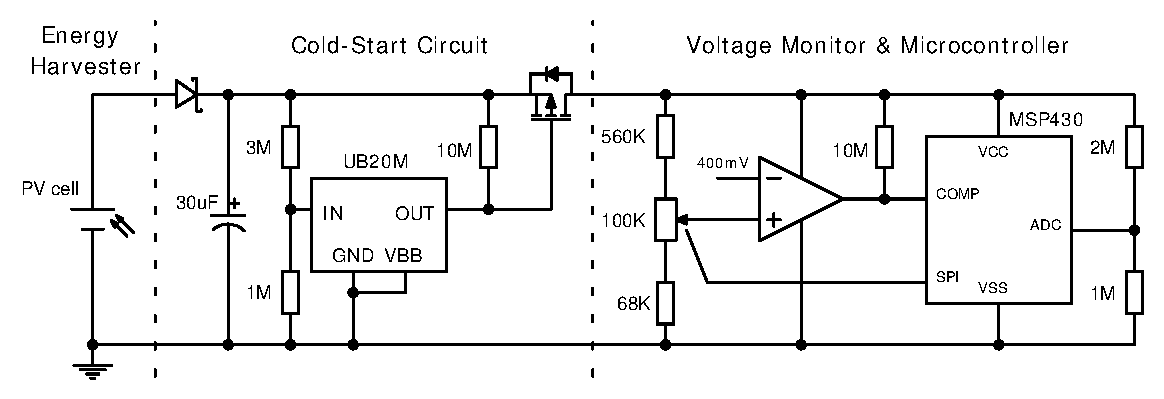
\includegraphics[width=7in]{ch5_repta/figures/circuit.pdf}
    \caption{System circuit. }
    \label{fig:schematic}
\end{figure*}

\newpage
\section{Implementation}

\begin{itemize}
    \item Overview
    \item Circuit
    \item Modules used in MSP430 
    \item State Saving and Restoring Algorithm
    \item Usage
\end{itemize}



\newpage
\section{Experimental Evaluation}

\subsection{Benchmark and Comparisons}

Benchmark: 

\begin{itemize}
    \item AES encryption
    \item AES decryption
    \item RF transmission
    \item UART send
    \item DMA (a very lightweight/efficient task, probably not ideal for the reliability test)
\end{itemize}

Comparisons:

DEBS, Samoyed (later), Plain C (for evaluating overheads)

We may temporarily overlook Samoyed as its implementation is a bit more complex and its threshold setting is unclear. 
Samoyed scales down the atomic task if it fails to complete (but never scale back). 
It uses an "energy profiler" in previous work to test the whether the smallest scale of all peripheral tasks and randomized inputs can successfully complete. 
They suggested it is appropriate to set an energy capacity that can run the smallest scale of an operation for hundreds of times in one energy cycle. 
Hence, it does not look for a threshold for a task with a specific configuration, but instead its aim is to minimize the chance of non-termination in practice by giving a high margin.

\subsection{Profiling Accuracy}

Question: How does our profiling approach perform in terms of accuracy?

Accuracy compared to manual measurement.

Figure shows:
\begin{itemize}
    \item Profiling results (average of 10)
    \item Each profiling reading (range)
    \item Dynamic threshold (Perhaps add horizontal lines as configurable thresholds in figures)
    \item Actual voltage drop (average of 5 manual readings)
\end{itemize}

\begin{figure}[t]
    \centering
    \begin{tikzpicture}
        \begin{axis}[
            width=1.0\columnwidth,
            height=5cm,
            ybar,
            xtick distance=1,
            ymin=0,
            ymax=60,
            xlabel=Test ID,
            ylabel=Profiled voltage droop (mV)
            ]
            \addplot
                plot [black,fill=white, error bars/.cd, y dir=both, y explicit]
                table [x=number, y=v_mean, y error plus=error_plus, y error minus=error_minus, col sep=comma] {ch5_repta/figures/dma_profiling/dma_profiling.csv};
            
            \coordinate (A) at (axis cs:1,45);
            \coordinate (O1) at (rel axis cs:0,0);
            \coordinate (O2) at (rel axis cs:1,0);
            \draw [black,sharp plot,dashed] (A -| O1) -- (A -| O2);
            % \addlegendentry{Constant Value}
        \end{axis}
    \end{tikzpicture}
    \caption{DMA profiling.}
    \label{fig:dma_profiling}
\end{figure}
\begin{figure}[!t]
    \centering
    \begin{tikzpicture}
    \begin{axis}[
        width=1.0\columnwidth,height=5cm,
        ybar,
        xtick distance=1,
        % enlarge x limits=0.3,
        ymin=0,
        ymax=300,
        xlabel=Test ID,
        ylabel=Profiled voltage droop (mV)
        ]
        \addplot
            plot [black, fill=white, error bars/.cd, y dir=both, y explicit]
            table [x=number, y=v_mean, y error plus=error_plus, y error minus=error_minus, col sep=comma] {ch5_repta/figures/aes_profiling/aes_profiling.csv};
        
        \coordinate (A) at (axis cs:1,266);
        \coordinate (O1) at (rel axis cs:0,0);
        \coordinate (O2) at (rel axis cs:1,0);
        \draw [black,sharp plot,dashed] (A -| O1) -- (A -| O2);
        % \addlegendentry{Constant Value}
    \end{axis}
    \end{tikzpicture}
    \caption{AES profiling.}
    \label{fig:aes_profiling}
\end{figure}
\begin{figure}[!t]
    \centering
    \begin{tikzpicture}
        \begin{axis}[
            width=1.0\columnwidth,
            height=5cm,
            ybar,
            xtick distance=1,
            ymin=0,
            ymax=750,
            xlabel=Test ID,
            ylabel=Profiled voltage droop (mV)
            ]
            \addplot
                plot [black,fill=white, error bars/.cd, y dir=both, y explicit]
                table [x=number, y=v_mean, y error plus=error_plus, y error minus=error_minus, col sep=comma] {ch5_repta/figures/uart_profiling/uart_profiling.csv};
            \coordinate (A) at (axis cs:1,652);
            \coordinate (O1) at (rel axis cs:0,0);
            \coordinate (O2) at (rel axis cs:1,0);
            \draw [black,sharp plot,dashed] (A -| O1) -- (A -| O2);
            % \addlegendentry{Constant Value}
        \end{axis}
    \end{tikzpicture}
    \caption{UART profiling.}
    \label{fig:uart_profiling}
\end{figure}

\subsection{Reliability with Dynamic Energy Consumption}

Question: Can it still make forward progress correctly with changes (as listed below) while other SoA approaches can't? 

Number of failures?

Cases of changes and experiments:

\subsubsection{New devices / operations (once)}

- Show the voltage trace that illustrates how it profiles and adapts on new devices or new operations. 

\subsubsection{Variability in capacitance due to ageing / tolerance (slowly changing)}

- Profile the tasks for DEBS with the target end voltage at 1.8V (need explanation on this) and 30uF capacitance. 

- Build a capacitor bank with a better granularity. The potential testing range of capacitance should be 20-30uF, so we probably use a combination of 2x10uF + 10x1uF capacitors, with some 0.1uF capacitors where necessary. 

- Decrease the capacitance step by step. Record the capacitance where DEBS fails, the adaptive thresholds, and a voltage trace that shows what happens. 

\subsubsection{Variability in peripheral configurations (single threshold for a rarely/slightly-changing configuration, multiple thresholds for frequently-changing configurations)}

- Profile the tasks for DEBS with the target end voltage at 1.8V and a "default" configuration. 
    
- Presumably DEBS can only complete the tasks with configurations that consumes the same or less energy as it was profiled, while OPTA adapts the threshold. 

\subsubsection{Variability in the amount of data to process (fast changing, but perhaps could be an unsuitable test case for reliability as it should violate the API requirement to make it fail)}
    
- This would be similar to the capacitance test but with a less granularity needed.


\subsection{Efficiency}

Question: Does it run faster than other SoA approaches (make more progress under the same energy condition) under conditions that all approaches can make forward progress?

Comparisons: DEBS, Samoyed.

Test conditions:
    
- (1) A constant data size (2) Randomized data sizes (DEBS threshold configured for the largest data size)

- A few levels of input current

\subsection{Overheads}

- Current \& time overheads of profiling and adaptation (with a further breakdown according to sub-operations) compared to Plain C. 

Time is measured by GPIO signals, and current is calculated by measuring voltage droops. 

The energy/charge consumption can also be calculated. 

- Memory overhead. Check the section sizes of the compiled code. Compared it to a PlainC version and a Hibernus-like IC version.  

\subsection{Correctness of computational results (test its intermittent computing functionality, might not be important)}

Question: does it produce correct results from atomic functions across power failures?

Compare the output of our approach with intermittent supply vs Plain C solution with continuous supply. Use a computational workload probably, as an atomic function should be guaranteed to finish. 


\subsection{Case Study}

Apply the proposed approach on an application that includes multiple atomic operations and the device runs with dynamic energy consumption due to operating conditions. 

\section{Conclusions}


% \section{Motivation}

% \section{Background}
% \subsection{Atomic Tasks Handling in Intermittent Systems}
% \subsection{Capacitor Degradation}

% \section{Online Task Profiling and Threshold Adaptation}
% \subsection{System Architecture}
% \subsection{Software Routine}
% \subsection{Online Task Profiling}
% \subsection{Voltage Threshold Adaptation}
% \subsection{Task Overhead Models}
% \subsubsection{Constant Model}
% \subsubsection{Linear Model}

% \section{Implementation}
% \subsection{Hardware}
% \subsection{Software}

% \section{Evaluation}
% \subsection{Experiment Setup}
% \subsubsection{Power Supply}
% \subsubsection{Benchmark}
% \subsection{Correctness}
% \subsection{Run Time}
% \subsection{Energy}
% \subsection{Memory Overhead}
% \subsection{Coping with Capacitor Degradation}

\section{Summary and Discussion}